% !TEX TS-program = pdflatex
% !TEX encoding = UTF-8 Unicode

\chapter{Data Preparation} \label{chapter:data_preparation}


\section{Cases and Controls}

To perform the association study, data from patients with T2D was collected. Both this data and the controls data is represented by \gls{VCF} files. The cases \gls{VCF} file contained 71 samples of the Portuguese patient's exome. When all of them were merged in a single file, there were 267 475 variants, either \gls{SNP}s or \gls{INDEL}s. No data of patient medical records was used, since it is already known that features such as \gls{BMI} and age can be great predictors of diabetes. Adding these to any model severely improves its accuracy, but the point of this study is to only use genomic data, more specifically \gls{SNP}s, to both predict and find new markers for \gls{T2D}. 

Since in the cases file there was no information about sex, it was decided that the study would be conducted without this division. There are several diseases that have different risk metrics depending on sex, but for \gls{T2D}, these are mostly due to environmental factors. As such, and also to not reduce further the number of samples by dividing it, division by sex was not performed.

The control data was collected from the 1000 Genome Project. It's goals involve discovering the most possible structural variants in the human genome of most ethnicities with frequencies of at least 1 \%. This project was able to collect 2504 samples from 26 populations, with at least 4x genome coverage, genotyped with high accuracy \cite{10002012integrated}. One of those populations is the IBS, which is short for Iberian populations in Spain. Considering all the case samples are of Portuguese patients, the closest ethnic group possible was selected, to avoid bias in data that would eventually lead to differentiation of populations instead of T2D. The number of samples gathered from this study were 107. The data is divided by chromosome, with gzip compressed files ranging from 200 MB to 2 GB, totalling 17.4 GB of compressed data. When uncompressed, these files reach at least 500 GB of storage, containing over 80 million variants across the genome.

The cases \gls{VCF} file offers numerous information of the variants, such as allele count in genotypes, total number of alleles in called genotypes, allele frequencies and so on. But the most important and the one that is going to be the most used is the GT field, which indicates the genotypes themselves. When making a call, short reads translate the information of two chromosomes. By using figure \ref{hom_het} as reference, and considering B as the REF allele, if most of the reads show a "B", it is genotyped as Homozygous by REF. If most show "b", it is considered homozygous by ALT. Since in this case, the genotype is unphased, it is not possible to know which chromosome the allele refers to, so both "Bb" and "bB" are classified as heterozygous. The REF allele is the one with the highest allele frequency in the population.

\begin{figure}
	\centering
	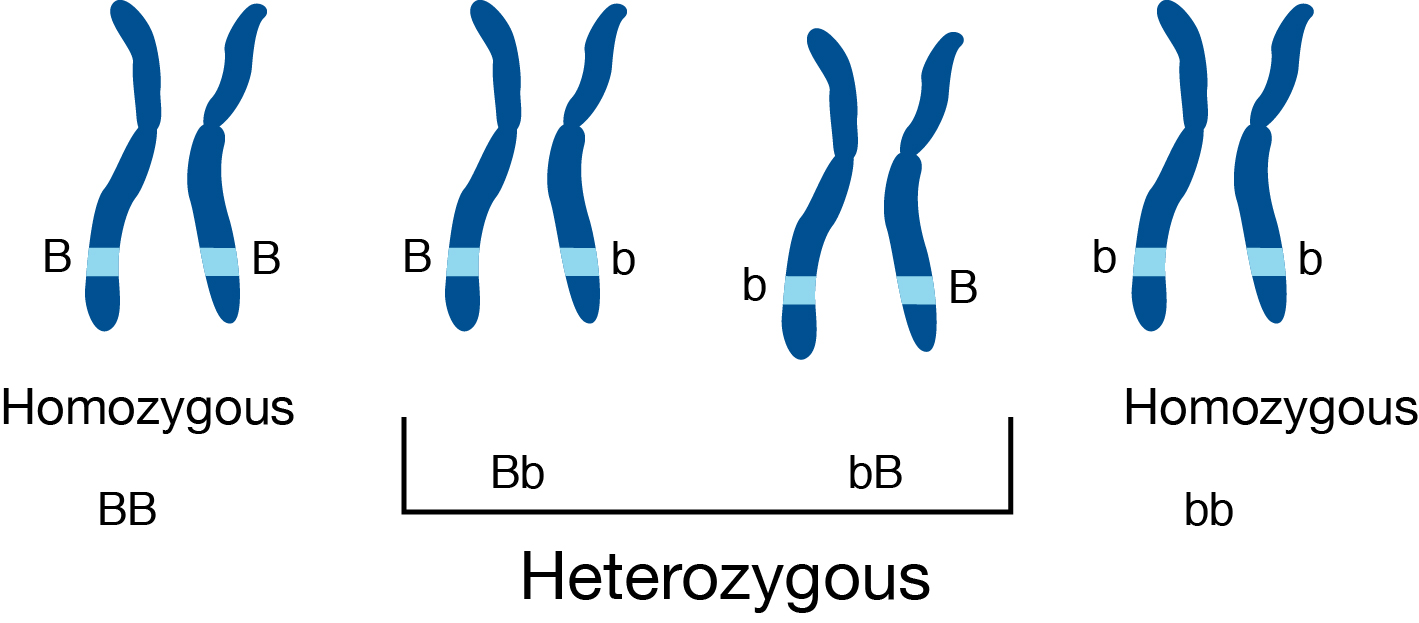
\includegraphics[width=4.5in]{../images/data_prep/hom_het.jpg}
	\caption{Visualization of possible genotypes for the structural variants. Adapted from public domain images at $https://www.genome.gov$ .} 
	\label{hom_het}
\end{figure}

In \gls{VCF} files, genotypes are represented as 0/0 for homozygous by REF, 0/1 for heterozygous, and 1/1 for homozygous by ALT. This needed to be translated in a way Machine Learning algorithms could interpret. To do so, a final structure of samples by variants is attained, where 0/0's are represented by 0's, 0/1's by 1's and 1/1's by 2's. The translation for \gls{SNP}s with more than 1 ALT allele can be seen in the table \ref{tab:genotypes}.

\begin{table}[h]

	\begin{tabular}{|c|c|>{\centering}p{.9cm}|>{\centering}p{.9cm}|>{\centering}p{.9cm}|c|}
		\hline                
		GT  & Translation  \\ 
		\hline
		0/0 & 0               \\
		0/1 & 1               \\
		1/1 & 2               \\
		0/2 & 3               \\
		1/2 & 4               \\
		2/2 & 5               \\
		0/3 & 6               \\
		... & ...             \\
		\hline
	\end{tabular} \\ \vskip .5cm
 	\caption{Translation of the genotypes (GT) of the VCF file to standard samples by variant dataset, for SNPs with several ALT alleles. }
 	\label{tab:genotypes}  
\end{table}

\section{Cases Quality Control}

The controls data from the 1000 Genome Project is already guaranteed to be of very high quality. However, it is important to analyse the cases dataset quality to ensure the confidence level that is put into it. If we're not confident of the quality of the dataset, several measures have to be taken to ensure results are not biased by wrong genotypes.

To analyse the quality of the cases dataset, a tool developed by Illumina called hap.py ($https://github.com/Illumina/hap.py$) was used. This tool produces solid comparison metrics between two \gls{VCF} files or one file and a reference genome. Since different genotyping methods can produce different ways of representing the structural variants, this comparison is not as straight forward as one might think. Hap.py besides solving these issues, counts \gls{SV} types and produces quality metrics for them. However, when comparing files, it was noted that the tool only compared the first exome to the reference. This happens because it was built not considering multi-sample \gls{VCF} files. As such, genotype accuracy metrics are not complete, but others such heterozygous to homozygous and transition to transversion ratios are still informative. The het/hom ratio is usually 2:1 for \gls{WGS} and lower for \gls{WES}. In the TsTv ratio, transitions are interchanges from purines or pyrimidines, and transversions involve interchanges of purines to pyrimidines or vice-versa. The expected proportion for this ratio is 2.1 for \gls{WGS} and higher (up to over 3) for \gls{WES}. The metrics for the first exome can then be observed in table \ref{tab:quality}. These were performed using the Platinum Genomes as the Gold Standard \gls{VCF} file.

\begin{table}[h]
	
	\begin{tabular}{|c|c|c|c|c|c|>{\centering}p{.9cm}|>{\centering}p{.9cm}|>{\centering}p{.9cm}|c|}
		\hline                
		Type  & Total Count & Truth het/hom & het/hom & Truth TsTv & TsTv \\ 
		\hline
		INDEL & 3449  & -    & - & 1.22 & 3.68         \\
		SNP	  & 49073 & 1.51 & 1.68 & 2.09 & 2.44      \\
		\hline
	\end{tabular} \\ \vskip .5cm
	\caption{Total count of \gls{INDEL}s found on the Gold Standard Platinum Genomes, and truth and cases dataset het/hom and TsTv ratios. The counts are much lower than the total variants because these are the ones found in the truth set.}
	\label{tab:quality}  
\end{table}

The het/hom ratio is slightly lower than 2:1 and the TsTv ratio is higher than the golden standard both because the dataset is of \gls{WES}, which is the expected.



\section{Dataset Construction}

As of this point, there are two separate datasets with very distinctive number of variants. As such, it is necessary to merge them in a single file, guaranteeing the most possible number of variants in the final file. 

This process is started by assembling the existing variants on the cases files and looking them up on the enormous chromosome files of the controls data. After all the possible variants are identified, their genotypes are extracted in the exact same way it was performed for the cases data. When lining up variants from both datasets, it was verified if their REF and ALT alleles matched. Those who did not were discarded. After it, 181 691 common variants were found between the two sets, which allowed to assemble them. 

To finalize the data clean up, missing values needed to be handled. The cases file had a rate of 22\% missing genotypes. This was improved when cases and controls were combined, but it was still a pressing issue. To solve it, every feature containing more than 10\% missing genotypes was removed. The remaining ones with only a few data points missing were imputed utilizing the most frequent value in that column. This leads to a final total of 168 432 variants. A final "labels" column was added with 0's representing control samples and 1's representing the cases.

It is important to note that, although ethnicities are the most similar possible, cases and controls were most likely acquired by different sequencers which might introduce bias differentiating them. The number of samples and variants can be seen in the table \ref{tab:numb_vars}.

\begin{table}[h]
	
	\begin{tabular}{|c|c|c|>{\centering}p{.9cm}|>{\centering}p{.9cm}|>{\centering}p{.9cm}|c|}
		\hline                
		Dataset & Number of Variants & Number of samples\\ 
		\hline
		cases & 267 475  & 71       \\
		controls & 81 271 745 & 107     \\
		total & 181 691 & 178 \\
		imputed & 168 432 & 178 \\
		\hline
	\end{tabular} \\ \vskip .5cm
	\caption{Number of samples and variants at each stage of the data processing.}
	\label{tab:numb_vars}  
\end{table}

\section{From Variants to Genes}

Although the data quality holds up, it is also necessary to assume that the dataset might contain some noise. This means that some variants can be extremely good differentiating the classes we created, especially since there many more variants than samples. These might not necessarily be noise or wrongfully genotyped variants, but it is better to look at whole regions and combine them instead, since it reduces this risk.  

The reason why it is possible to infer information of variants from gene regions is thanks to Linkage Disequilibrium. As it can be seen on figure \ref{fig:LD}, by identifying regions of high \gls{LD} it is possible to attain information of several disease related \gls{SNP}s, even if they are not directly contained in the dataset.

\begin{figure}[h]
	\centering
	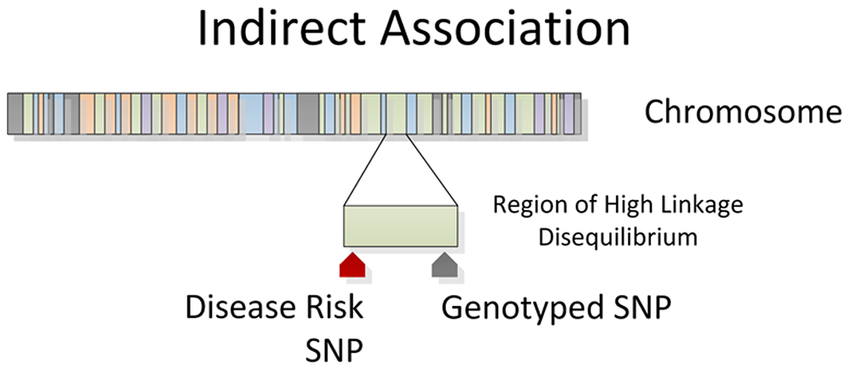
\includegraphics[width=\textwidth]{../images/data_prep/LD.png}
	\caption{Visualization of high Linkage Disequilibrium regions which allow for usage of genotyped \gls{SNP}s to infer disease risk \gls{SNP} \cite{bush2012genome}.} 
	\label{fig:LD}
\end{figure}

As such, it is critical to be able to extract information relative to which gene a variant belongs to, so it is possible to group them. This is one of the fastest and most meaningful ways of grouping variants, since directly performing tests of \gls{LD} between each variant would be extremely computationally heavy.

To do so, a package for R called BiomaRt was used, that allows to query the Ensembl database. It works essentially as a genome browser with information of genomics, evolution, transcriptional regulation, sequence variation and annotations of genes, alignments and disease data. By querying the respective genes for the available variants, it is then possible to build a dictionary for an easy mapping of variants to genes. However, sometimes this querying cannot retrieve gene information because the variant is still not mapped. When this happened, a note is attached to the variant, but the analysis progresses with these marked as having no gene.
